\documentclass[../main.tex]{subfiles}
\begin{document}
%\chapter{Results}\label{ch:O}
\section{Second order}
Since the Suzuki-Trotter product formula is only an approximation to solve the time dependent Schr{\"o}dinger equation, the error involved depends on the time interval $\tau$ - the time step at which the evolution is computed (see Eq. \ref{eq:b17}). 

Thus, for checking if the evolution using the Suzuki-Trotter product formula is indeed second order, the dependence of the error should be verified to be quadratic in $\tau$, in accordance with Eq. (\ref{eq:b18}). 
\begin{figure}[H]
\centering 
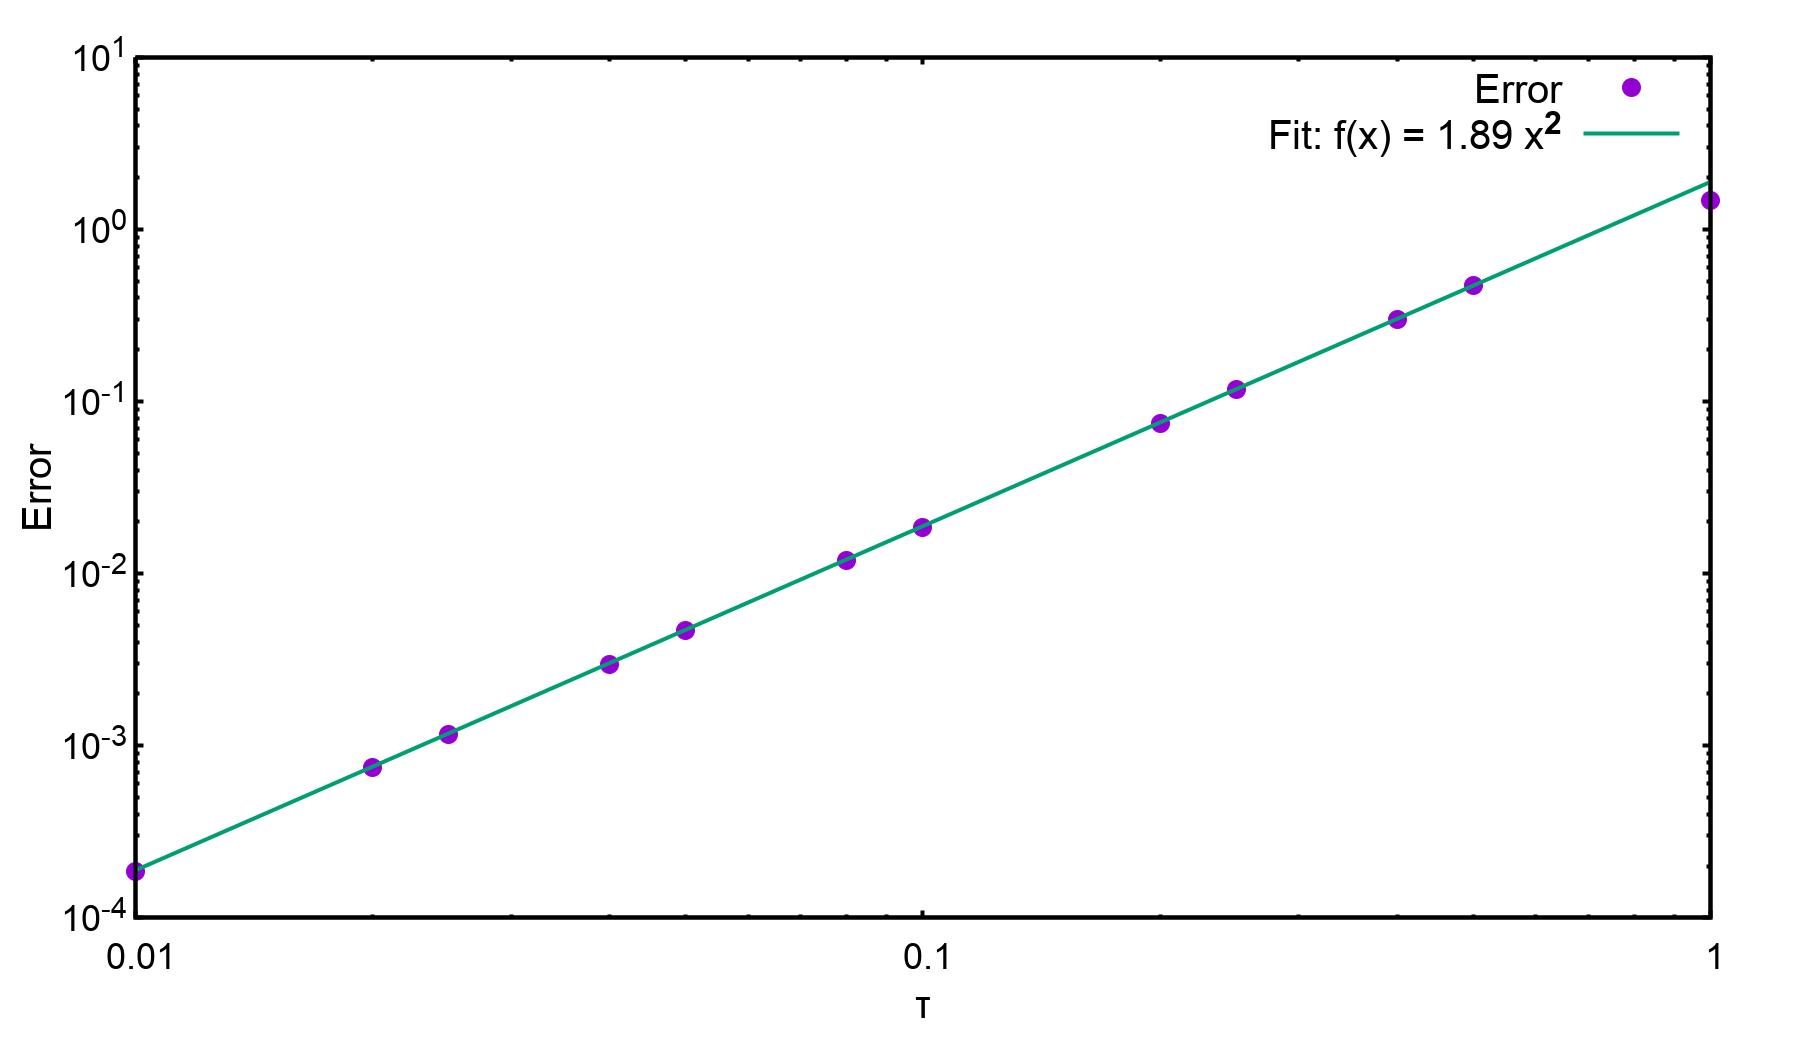
\includegraphics[scale=0.2]{Error.png}
\caption{The error in Suzuki-Trotter formula relative to the full diagonalization method. The involved error grows quadratically in $\tau$.}
\label{fig:o1}
\end{figure}
Since the dependence of the error on $\tau$ can be approximated to be linear in the log scale, as shown in Fig. (\ref{fig:o1}), the simulation implementing TDSE can be trusted to be following the second order Suzuki-Trotter product formula.

For the course of this thesis, we worked with 8 spin and 12 spin 2-local problems. The first set had 91 unique problems, while the second set had 1000 such problems. All the problems had a predetermined unique ground state, and only one avoided crossing between the ground and the first excited state. The 8 spin problems had 9 pair-wise couplings, while the 12 spin problems had 13 such couplings. The success probability was then obtained by calculating the overlap between the known ground state and the final state resulting from the code performing product evolution. Furthermore, for determining the energy spectra for specific problems, exact diagonalization method was employed.

This chapter focusses on the results obtained for original Ising Hamiltonian, i.e. in the absence of any triggers. 


For every problem belonging to the set, three annealing times were chosen to calculate the success probability. These correspond to $T_A \in \{ 10,100,1000 \}$. For a given $T_A$, the resulting success probability is a function of the minimum energy gap, $\Delta_{min}$, between the ground and the first excited state. For a fixed $T_A$, the success probability is expected to decrease with decreasing $\Delta_{min}$, if the evolution of the state is adiabatic. Thus, the hardness of a problem can be estimated by its minimum energy gap.\\


As the first example, considered here is problem number 733, that was noted to have high success probability, i.e., $p=0.9944$ for $T_A=100$. Fig. (\ref{fig:o2}), shows the energy spectrum for this problem. $\Delta_{min}$ was found to be 0.4407 in this case.  Also plotted in the figure are the energy expectation values for the instantaneous state obtained for the three different annealing times.
\begin{figure}[H]
\centering 
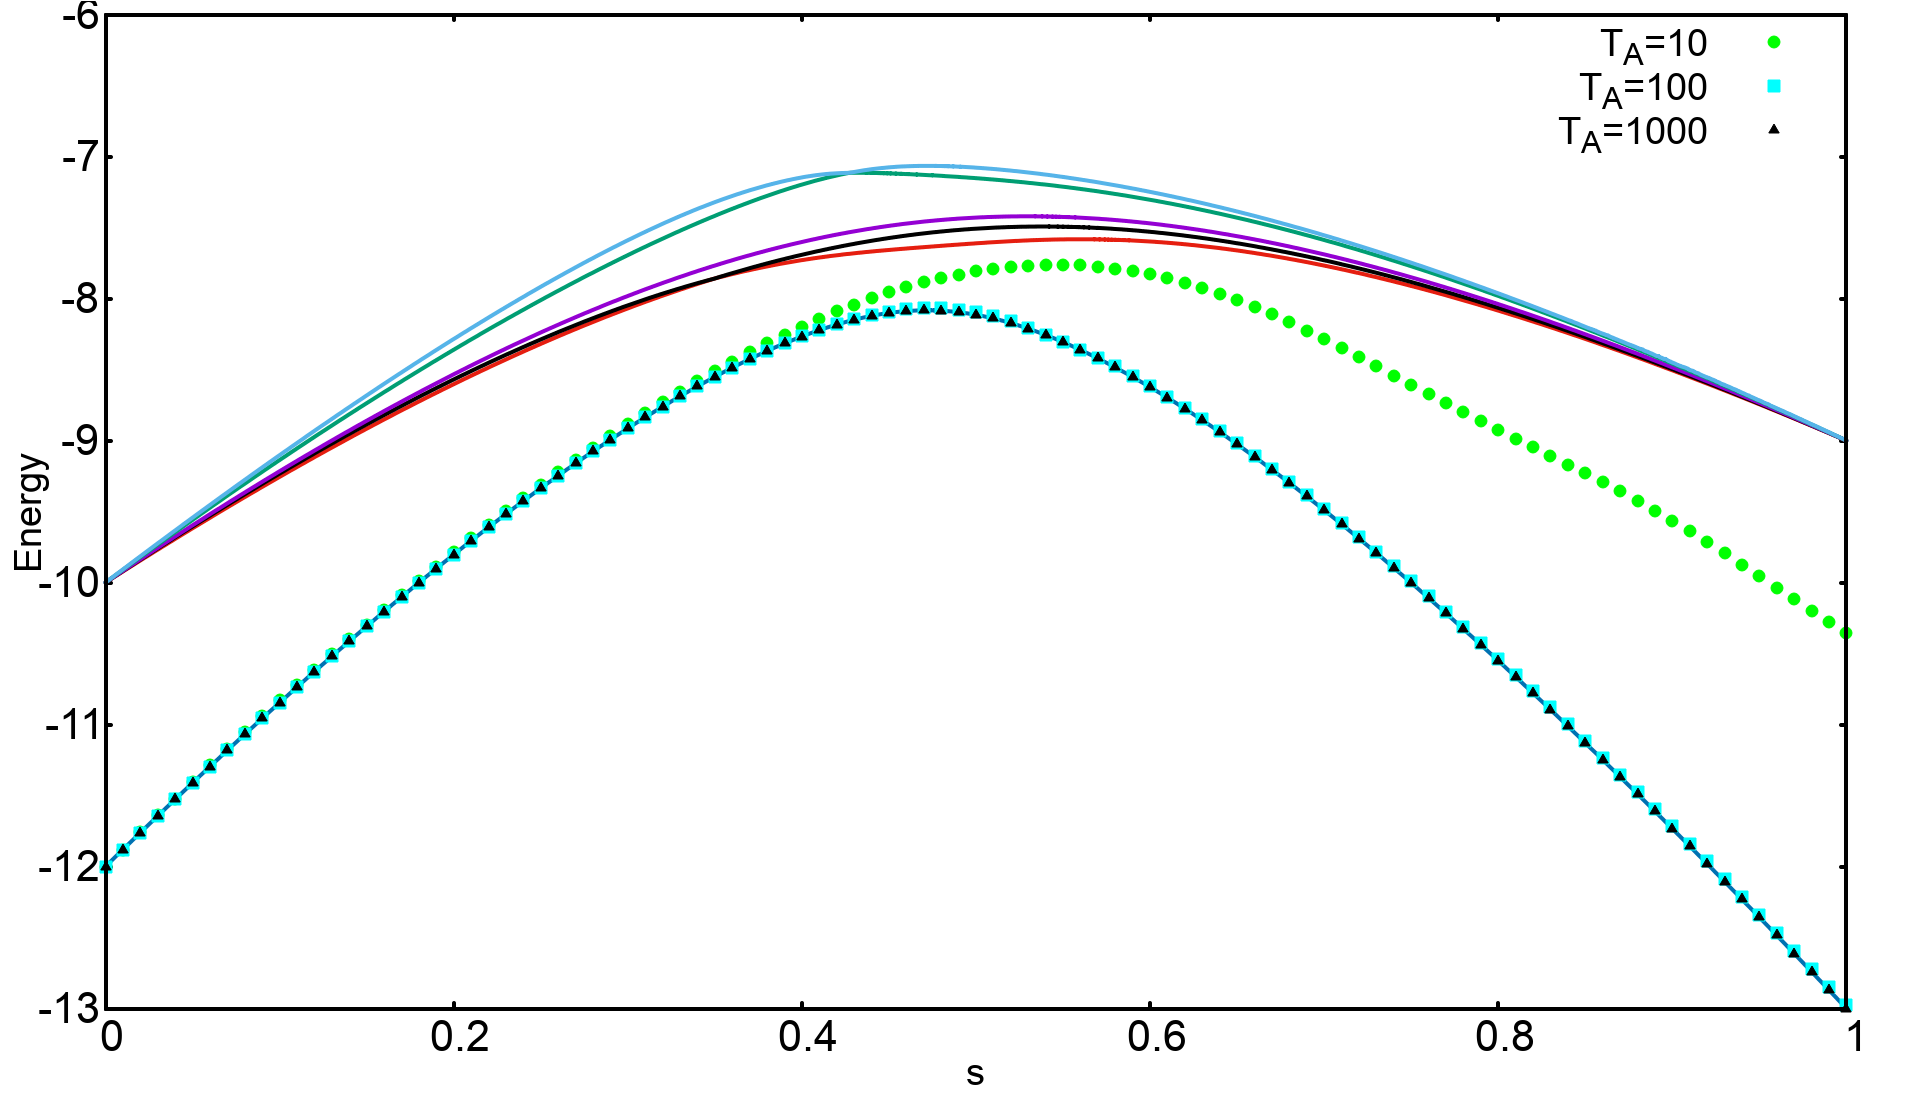
\includegraphics[scale=0.24]{733_s12_O.png}
\caption{The energy spectrum for problem 733, with energy expectation values for the instantaneous state, corresponding to three annealing times. For $T_A$=100, $p$ was found to be 0.9944, while $\Delta_{min}=0.4407.$}
\label{fig:o2}
\end{figure}

As expected, the overlap of the final state with the ground state of the problem Hamiltonian increases on increasing the total annealing time in Fig. (\ref{fig:o2}).\\

Secondly, problem number 950, with small success probability, $p= $0.0146 at $T_A=100$, was chosen. Fig. (\ref{fig:o3}) shows the energy spectrum and the energy expectation values for the instantaneous state corresponding to three annealing times, for this problem. It should be noted, that the minimum gap in this is much smaller than in problem 733, and has a value of $\Delta_{min} = 0.0312$. This explains the decrease in success probability for the same annealing times.\\
\begin{figure}[H]
\centering 
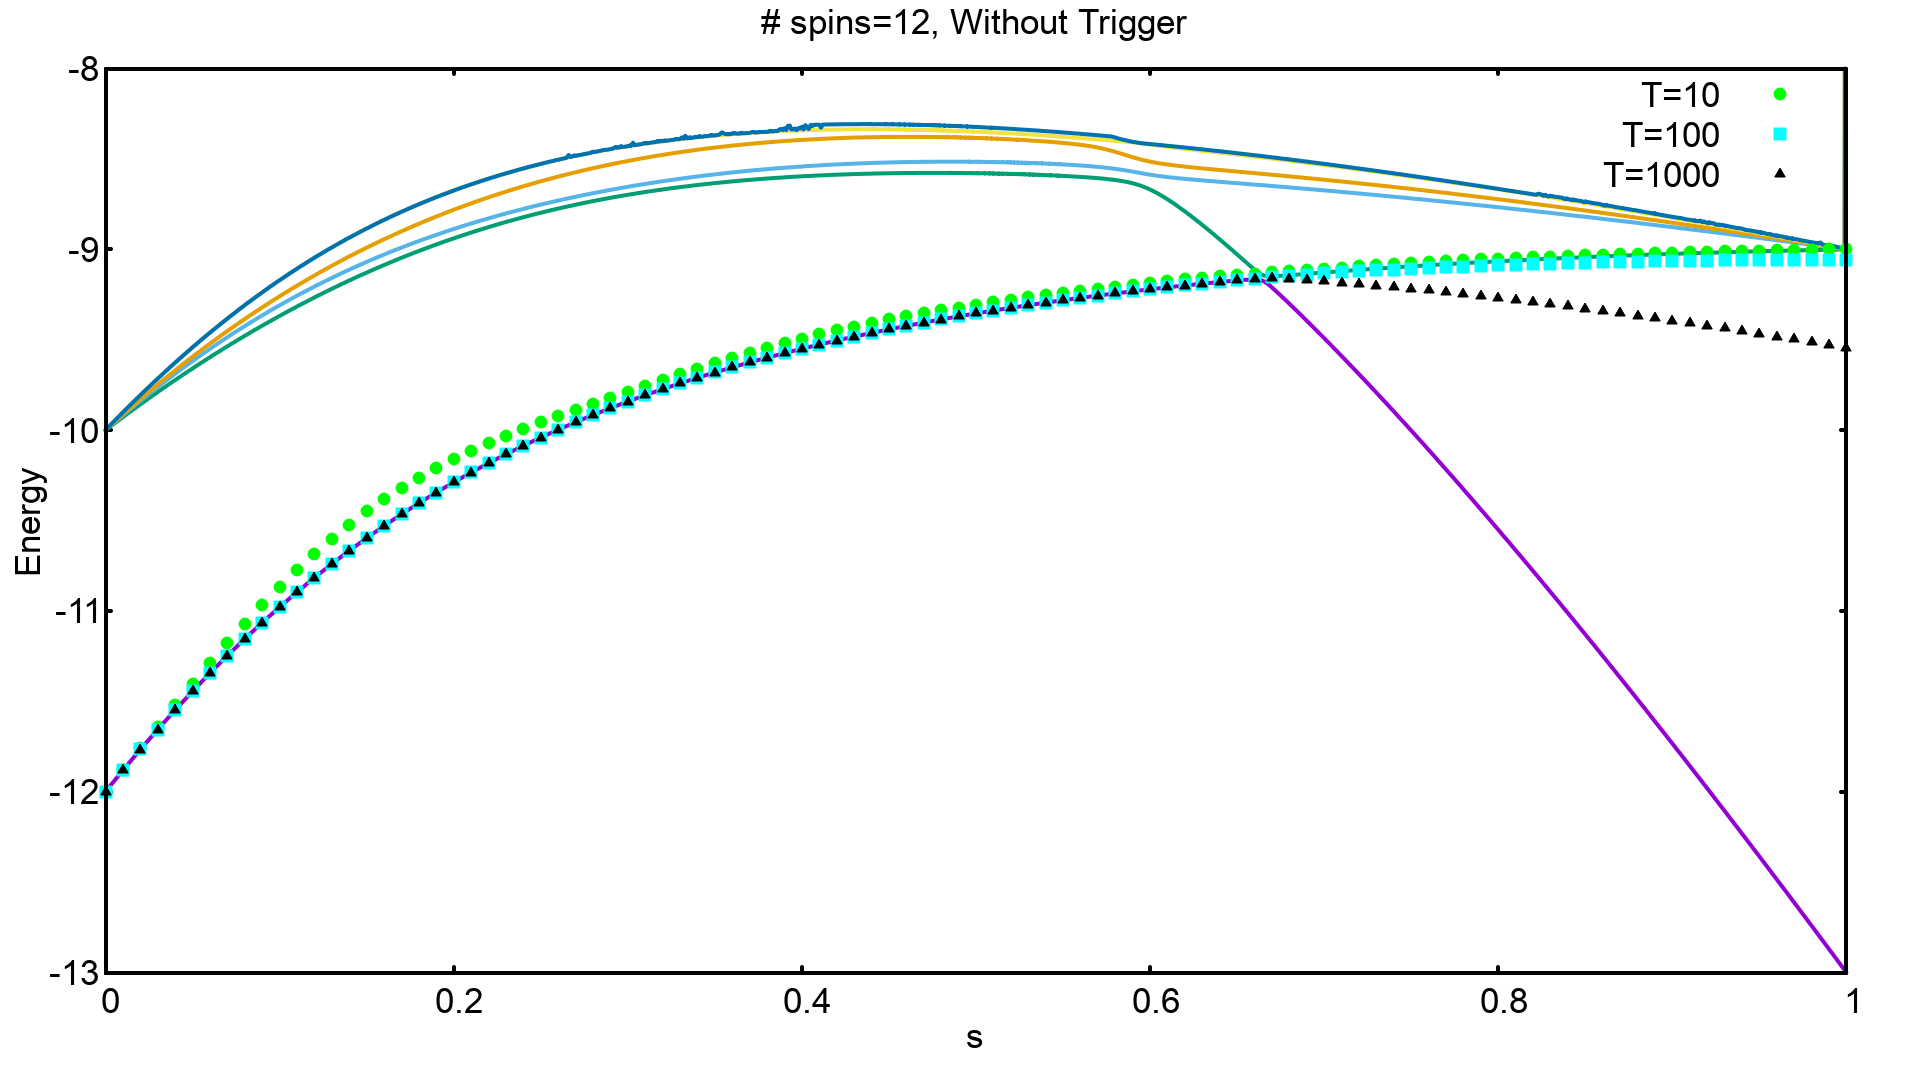
\includegraphics[scale=0.24]{950_s12_O.png}
\caption{The energy spectrum for problem 950, with energy expectation values for the instantaneous state, corresponding to three annealing times. For $T_A$=100, $p$ was found to be 0.0146, while $\Delta_{min}=0.0312.$}
\label{fig:o3}
\end{figure}


As the third case, problem number 528, with an intermediate success probability of $p=0.5199$ at $T_A= 100$ was studied. For this case too, the energy spectrum and the energy expectation values for the instantaneous state, corresponding to the three annealing times were determined, as is shown in Fig. (\ref{fig:o4}). The value of minimum gap was $\Delta=0.1573$ for this problem, which is intermediate to the above two cases. 
\begin{figure}[H]
\centering 
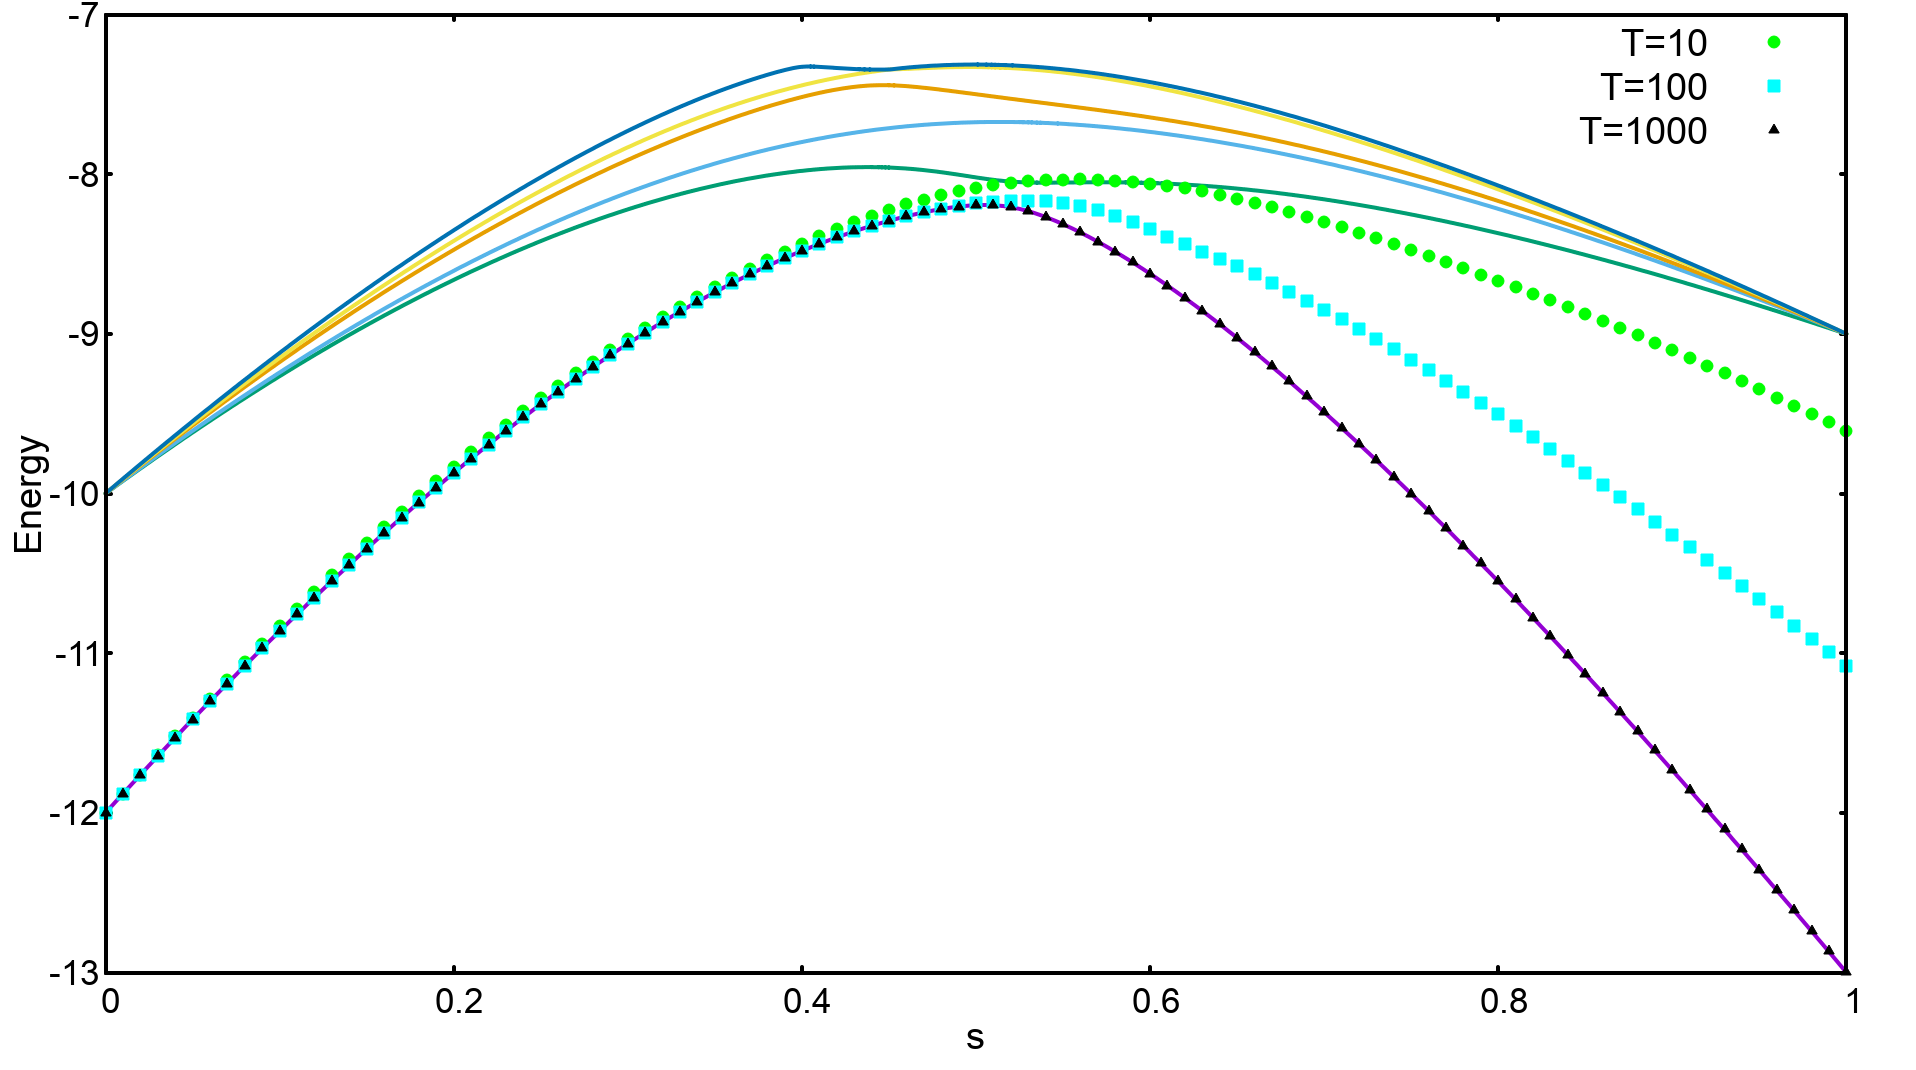
\includegraphics[scale=0.24]{528_s12_O.png}
\caption{The energy spectrum for problem 528, with energy expectation values for the instantaneous state, corresponding to three annealing times. For $T_A$=100, $p$ was found to be 0.5199, while $\Delta=0.1573.$}
\label{fig:o4}
\end{figure}

\begin{comment}
The main feature of difference between the 12-spin and 8-spin problems is that the minimum energy gaps of the 8-spin problems were found to be larger than those of 12-spin problems. This can be understood with the help of Eq. (\ref{eq:b10}), where the minimum gap is expected to close exponentially with increasing N. Even the gap corresponding to the case with smallest success probability in 8-spin problems (the smallest energy gap amongst 91 8-spin problems, $\Delta_{min}=0.4725$) is still larger than the the gap corresponding to the case with largest success probability in 12-spin problems (the largest energy gap amongst 1000 12-spin problems, $\Delta_{min}=0.4407$). Therefore, even an annealing time of $T_A=100$ yields a large success probability for almost all 8-spin cases. 
\end{comment}


To obtain a rough estimate of the spread of the difficulty of the problems considered in this work, Fig. (\ref{fig:o8}) shows a plot of the distribution of the success probabilities for $T_A=100$, for all the problems in the set. The range of the success probability spreads from 0.014 for the most difficult cases, to approximately 1 for the relatively easier cases. The mode of the distribution was found to be 0.141 and 0.199, while the mean success probability was found to be 0.208. 
\begin{figure}[H]
\centering 
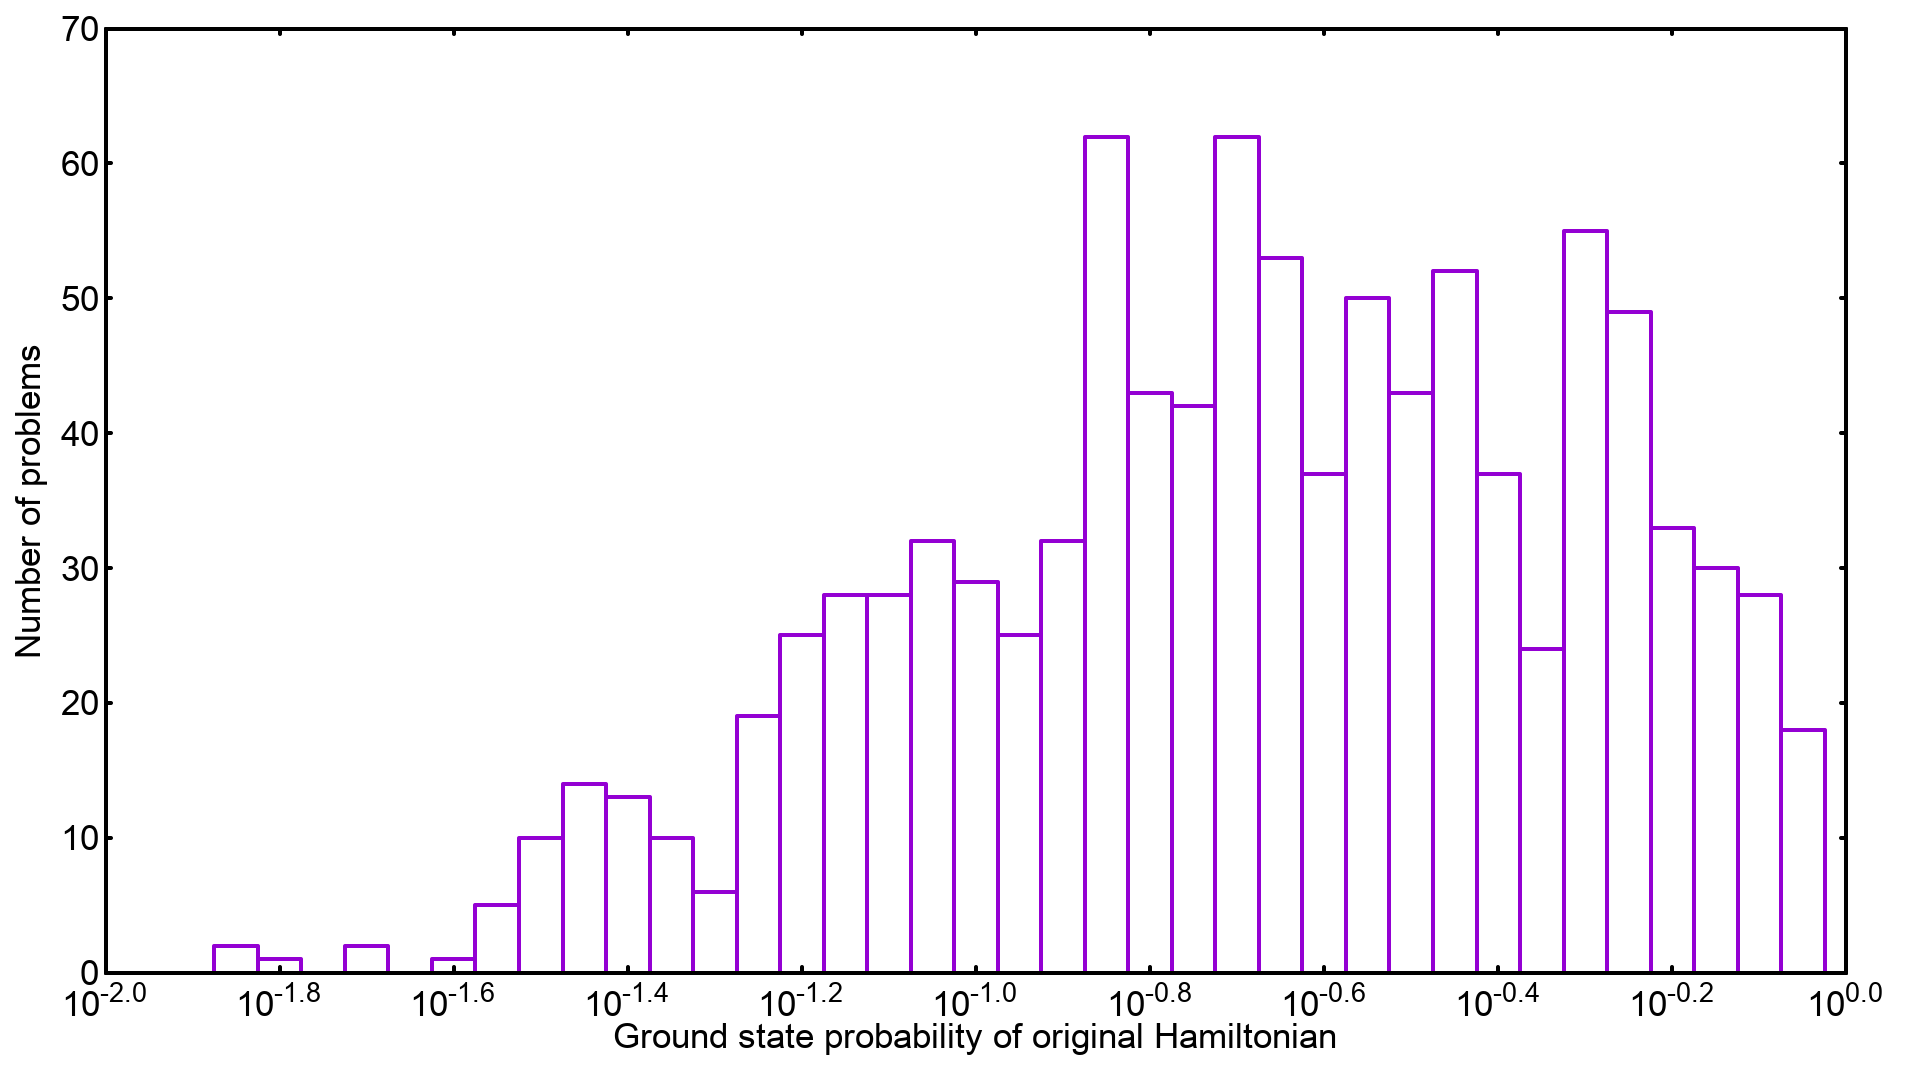
\includegraphics[scale=0.24]{O_s12_T100_g0.png}
\caption{Histogram for success probability of the Hamiltonians without any triggers for 1000 12-spin problems for $T_A$=100.}
\label{fig:o8}
\end{figure}

Finally, to check if the sweeping from the initial Hamiltonian to the final Hamiltonian is adiabatic, the success probability of all the 12-spin problems has been plotted in Fig. (\ref{fig:o10}).
\begin{figure}[H]
\centering 
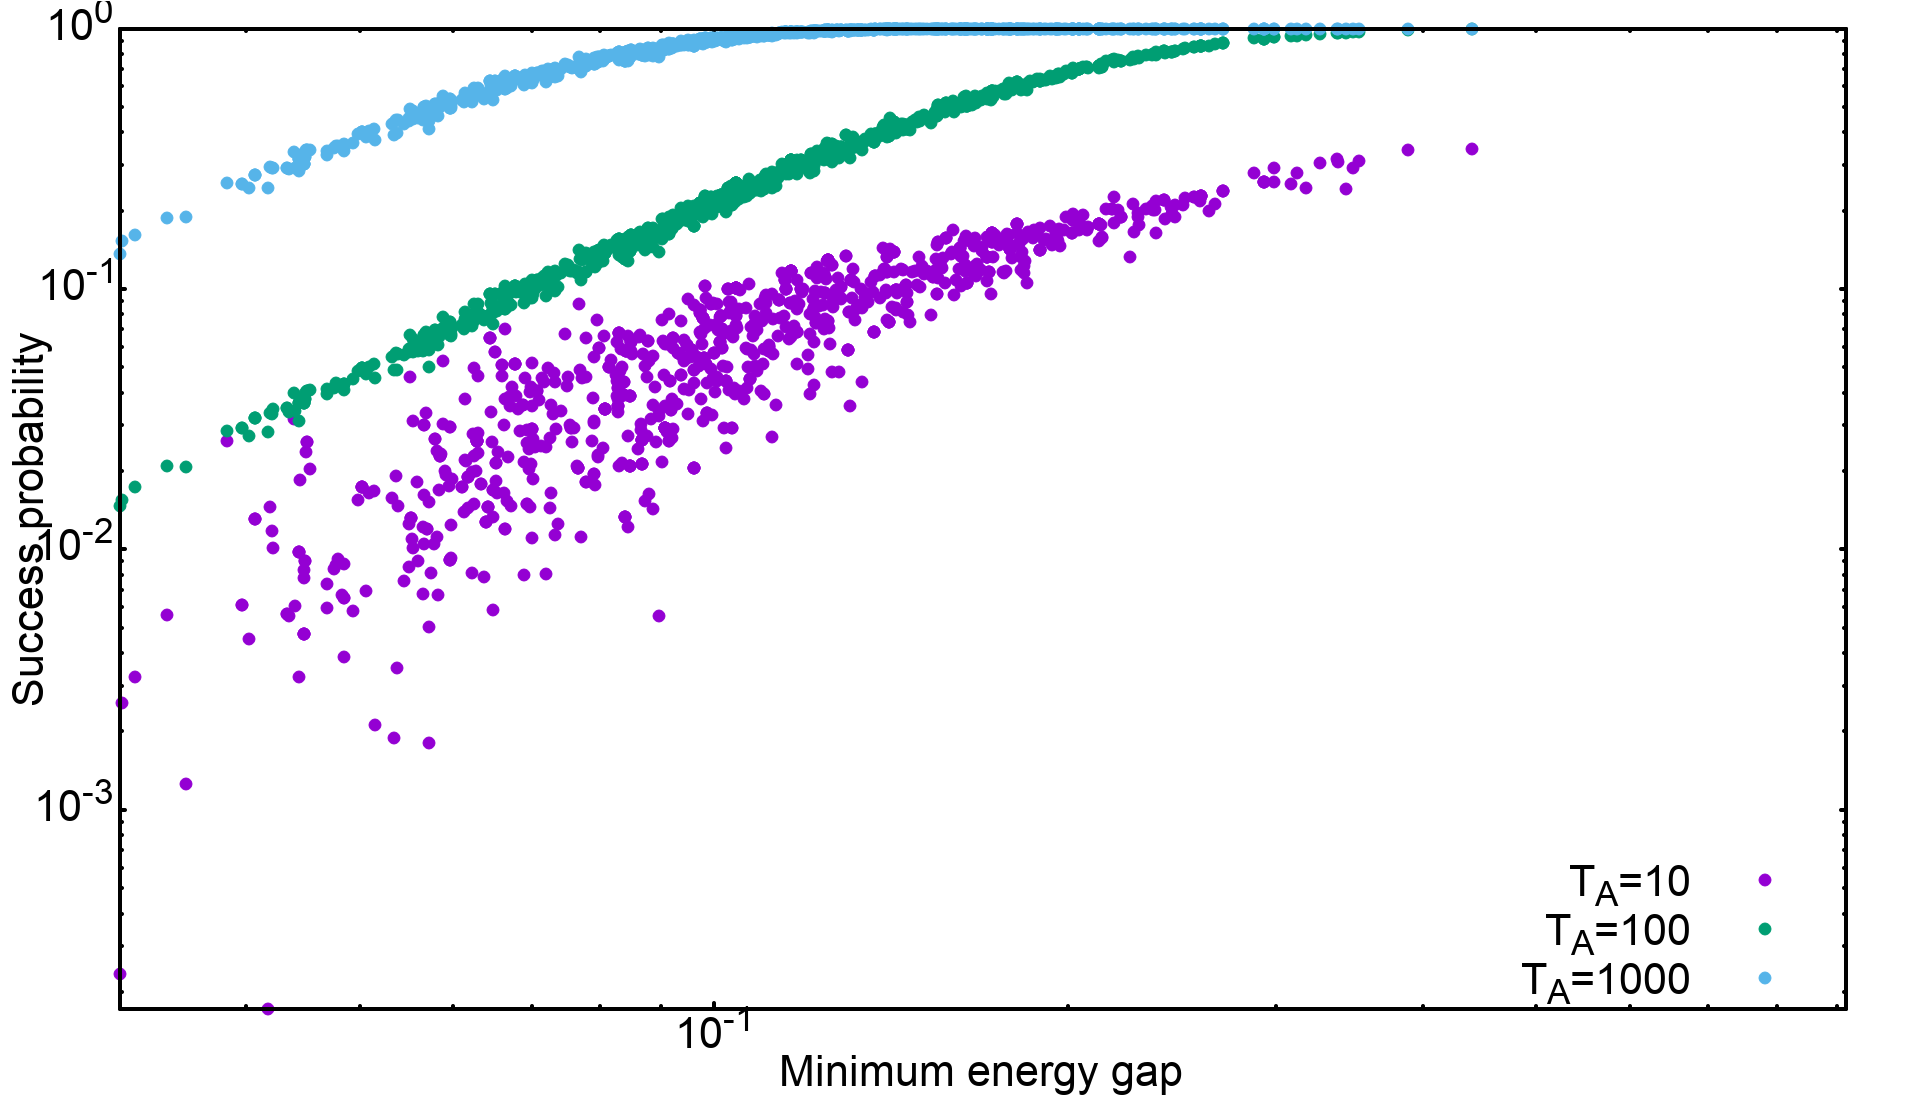
\includegraphics[scale=0.24]{GapVsSucc_s12_T10_100_1000.png}
\caption{Success probability Versus minimum energy gaps for all the 12-spin problems for annealing times of 10,100 and 1000.}
\label{fig:o10}
\end{figure}
From Eq. (\ref{eq:lz3}), the probability of ending in a state close to the ground state of the problem Hamiltonian should follow the Landau-Zener dependence on the minimum energy gap between the ground and first excited state of the Hamiltonian, if the evolution of the state is adiabatic. Since different problems belonging to the set correspond to different values of $\Delta_{min}$, the success probability for each problem, plotted against the respective minimum energy gap for a fixed annealing time, can give an estimate of the fraction of cases undergoing adiabatic evolution. More the scattering in the resulting curve, smaller is the fraction of problems following the adiabatic theorem. It can therefore be noted in Fig. (\ref{fig:o10}) that for $T_A$=10, the scattering is significantly larger than in the other two cases. It should additionally be observed that as the annealing time is increased, the success probability for a specific problem becomes successively larger. This suggests that as the annealing time is increased, the evolution of the state becomes adiabatic for more number of problems.


\end{document}